% The DV control loop: structure, equations, stability and measurements.
% Build: latexmk -pdf control_loop.tex   (pdfLaTeX, TikZ, pgfplots)
\documentclass[11pt,a4paper]{article}
\usepackage[margin=2.2cm]{geometry}
\usepackage[T1]{fontenc}
\usepackage{lmodern}
\usepackage{amsmath,amssymb}
\usepackage{booktabs}
\usepackage{siunitx}
\usepackage{xcolor}
\usepackage{tikz}
\usetikzlibrary{arrows.meta,positioning,fit,calc,shapes.geometric}
\usepackage{pgfplots}
\pgfplotsset{compat=1.18}
\usepackage[hidelinks]{hyperref}
\usepackage{cleveref}

\sisetup{detect-all, per-mode=symbol}
\definecolor{stan}{HTML}{C44E52}
\definecolor{pp}{HTML}{4C72B0}
\definecolor{fix}{HTML}{55A868}
\definecolor{bud}{HTML}{333333}
\newcommand{\vect}[1]{\boldsymbol{#1}}
\newcommand{\wrap}{\operatorname{wrap}}
\newcommand{\sat}{\operatorname{sat}}

\tikzset{
  blk/.style={draw, rounded corners=2pt, align=center, minimum height=9mm, inner sep=4pt, font=\small},
  pi/.style={blk, fill=pp!12},
  car/.style={blk, fill=gray!15},
  mcu/.style={blk, fill=fix!15},
  sig/.style={-{Latex[length=2mm]}, thick},
  lab/.style={font=\scriptsize, midway, fill=white, inner sep=1pt},
}

\title{The DV control loop\\[2pt]\large structure, equations, stability and measurements}
\author{IFS09 DV pipeline, branch \texttt{pipeline\_arm\_optimization}}
\date{14 November 2026}

\begin{document}
\maketitle

\begin{abstract}
This document describes the vehicle controller of the DV pipeline as it runs on the
Orange Pi~5 Plus (RK3588) and as it will move to the uDV STM32H7: where it sits in the
loop, every equation it evaluates, the delays around it, and the measurements behind its
settings. It also records two changes made on 14 November 2026. First, Stanley's
yaw-rate damping is now scaled by speed. The fixed gain closed a loop with gain
$1.4$ around a delay of about \SI{110}{\milli\second}, which oscillated at
\SI{4}{\hertz} in hardware-in-the-loop (HIL) runs; all 24 cones hit in the reference HIL
session were in Stanley missions. Second, a delay compensator was added and left off,
because with the corrected gain the remaining delay costs no tracking.
\end{abstract}

\tableofcontents
\newpage

%=====================================================================
\section{Where control sits}
%=====================================================================

\Cref{fig:arch} shows the pipeline on the RK3588. Each per-scan stage has its own A76
core. Control runs on core~7 with the odometry filter and the network interrupts. It
takes the path from planning, the pose from SLAM, the velocity from the odometry filter
and the big-orange cones from detection. Its command goes through mission control, which
relays it to the vehicle interface (the uDV on the car, the sim supervisor in HIL).

\begin{figure}[h]
\centering
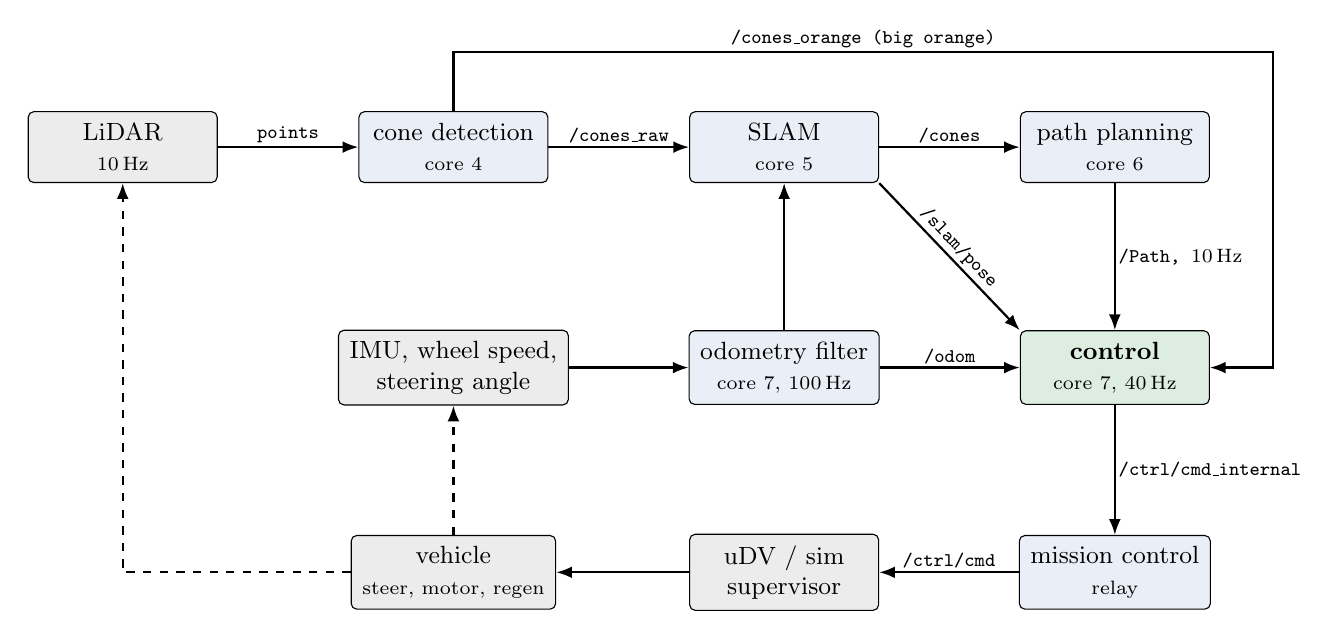
\begin{tikzpicture}[font=\small, tl/.style={font=\scriptsize\ttfamily, inner sep=1pt}]
  \tikzset{b/.style={blk, minimum width=24mm}}
  \node[car,b] (lidar) at (0,0) {LiDAR\\\scriptsize\SI{10}{\hertz}};
  \node[pi,b] (det) at (4.2,0) {cone detection\\\scriptsize core 4};
  \node[pi,b] (slam) at (8.4,0) {SLAM\\\scriptsize core 5};
  \node[pi,b] (plan) at (12.6,0) {path planning\\\scriptsize core 6};
  \node[car,b] (sens) at (4.2,-2.8) {IMU, wheel speed,\\steering angle};
  \node[pi,b] (odom) at (8.4,-2.8) {odometry filter\\\scriptsize core 7, \SI{100}{\hertz}};
  \node[pi,b, fill=fix!20] (ctrl) at (12.6,-2.8) {\textbf{control}\\\scriptsize core 7, \SI{40}{\hertz}};
  \node[car,b] (veh) at (4.2,-5.4) {vehicle\\\scriptsize steer, motor, regen};
  \node[car,b] (udv) at (8.4,-5.4) {uDV / sim\\supervisor};
  \node[pi,b] (mc) at (12.6,-5.4) {mission control\\\scriptsize relay};
  \draw[sig] (lidar) -- node[tl,above]{points} (det);
  \draw[sig] (det) -- node[tl,above]{/cones\_raw} (slam);
  \draw[sig] (slam) -- node[tl,above]{/cones} (plan);
  \draw[sig] (plan) -- node[tl,right]{/Path, \SI{10}{\hertz}} (ctrl);
  \draw[sig] (slam.south east) -- node[tl,sloped,above]{/slam/pose} (ctrl.north west);
  \draw[sig] (det.north) -- ++(0,0.75) -| node[tl,above,pos=0.25]{/cones\_orange (big orange)} ([xshift=8mm]plan.east) |- (ctrl.east);
  \draw[sig] (sens) -- (odom);
  \draw[sig] (odom) -- node[tl,above]{/odom} (ctrl);
  \draw[sig] (odom) -- (slam);
  \draw[sig] (ctrl) -- node[tl,right]{/ctrl/cmd\_internal} (mc);
  \draw[sig] (mc) -- node[tl,above]{/ctrl/cmd} (udv);
  \draw[sig] (udv) -- (veh);
  \draw[sig, dashed] (veh) -- (sens);
  \draw[sig, dashed] (veh.west) -| (lidar.south);
\end{tikzpicture}
\caption{The loop on the RK3588. Blue: processes on the Pi with their pinned cores
(\texttt{DV\_CPU\_PIN} in \texttt{deploy/rk3588.env}). Grey: the car or the sim. Dashed:
the physical loop back through the car.}
\label{fig:arch}
\end{figure}

\paragraph{Inside control.} \Cref{fig:inside} shows one \SI{40}{\hertz} tick. All of it is
\texttt{control\_cpp/src/control\_core.c}: plain C99 with \texttt{<math.h>} only, no heap,
no operating system and no ROS. The rclcpp node \texttt{control\_cpp/src/control\_node.cpp}
only converts messages. The Python package \texttt{control} is the reference: the tests
in \texttt{control/test/test\_control\_core\_c.py} hold the C code to it within
$10^{-9}$, piece by piece and over closed-loop runs of whole missions.

\begin{figure}[h]
\centering
\resizebox{\linewidth}{!}{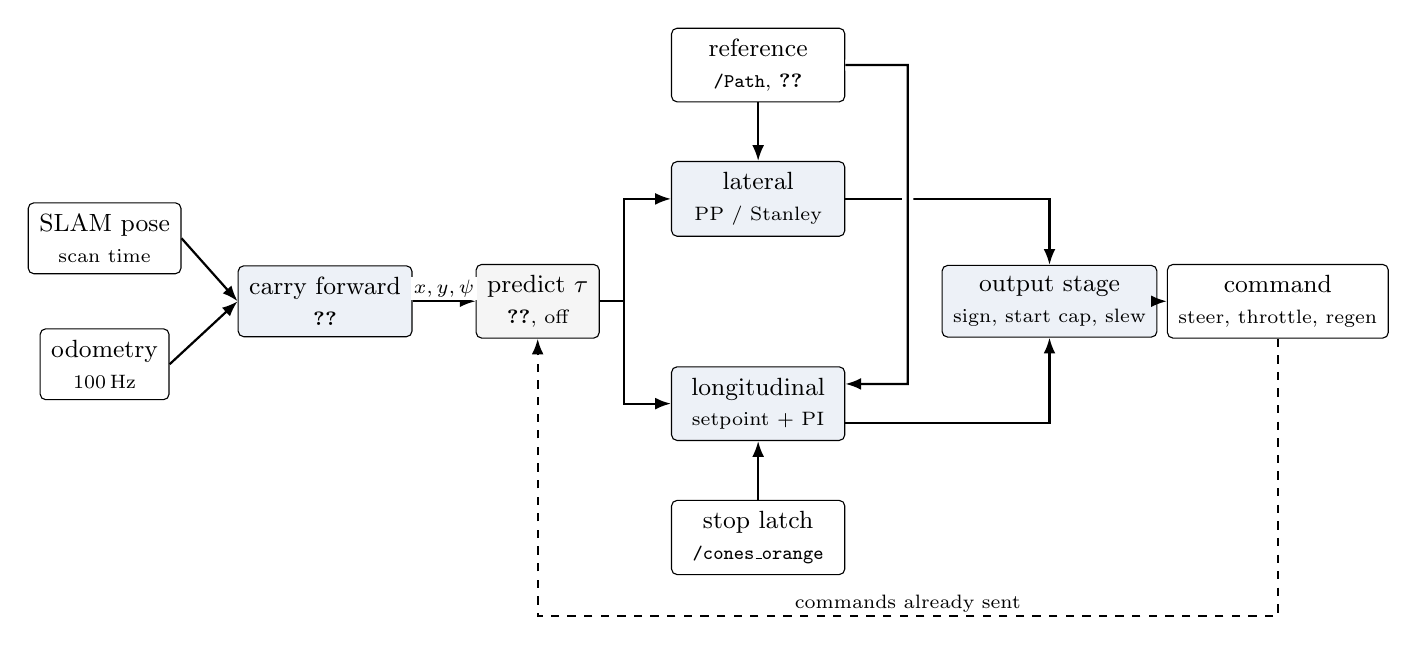
\begin{tikzpicture}[font=\small]
  \tikzset{b/.style={blk, minimum width=22mm}}
  \node[blk] (pose) at (0,0.8) {SLAM pose\\\scriptsize scan time};
  \node[blk] (odom) at (0,-0.8) {odometry\\\scriptsize \SI{100}{\hertz}};
  \node[blk, fill=pp!10] (proj) at (2.8,0) {carry forward\\\scriptsize \cref{eq:project}};
  \node[blk, fill=gray!8] (pred) at (5.5,0) {predict $\tau$\\\scriptsize \cref{eq:predict}, off};
  \node[b, fill=pp!10] (lat) at (8.3,1.3) {lateral\\\scriptsize PP / Stanley};
  \node[b, fill=pp!10] (lon) at (8.3,-1.3) {longitudinal\\\scriptsize setpoint + PI};
  \node[b] (ref) at (8.3,3.0) {reference\\\scriptsize \texttt{/Path}, \cref{eq:ref}};
  \node[b] (stop) at (8.3,-3.0) {stop latch\\\scriptsize \texttt{/cones\_orange}};
  \node[blk, fill=pp!10] (out) at (12.0,0) {output stage\\\scriptsize sign, start cap, slew};
  \node[blk] (cmd) at (14.9,0) {command\\\scriptsize steer, throttle, regen};
  \draw[sig] (pose.east) -- (proj.west); \draw[sig] (odom.east) -- (proj.west);
  \draw[sig] (proj) -- node[lab,above]{$x,y,\psi$} (pred);
  \draw[thick] (pred.east) -- (6.6,0);
  \draw[sig] (6.6,0) |- (lat.west); \draw[sig] (6.6,0) |- (lon.west);
  \draw[sig] (ref) -- (lat); \draw[sig] (stop) -- (lon);
  \draw[sig] (lat.east) -| (out.north);
  \draw[sig] ([yshift=-2.5mm]lon.east) -| (out.south);
  \draw[sig, preaction={draw, white, line width=4pt}] (ref.east) -| (10.2,-1.05) -- ([yshift=2.5mm]lon.east);
  \draw[sig] (out) -- (cmd);
  \draw[sig, dashed] (cmd.south) |- (5.5,-4.0) node[lab, pos=0.75, above]{commands already sent} -- (pred.south);
\end{tikzpicture}}
\caption{One control tick. The dashed path feeds the published commands back to the
delay predictor (\cref{sec:delaycomp}).}
\label{fig:inside}
\end{figure}

%=====================================================================
\section{Timing and delays}
%=====================================================================

\Cref{tab:rates} lists the rates and the delays measured in the HIL session
\texttt{hil\_v10\_conearray} (10 missions, \SI{4144}{\second}). Delays between two
signals come from the lag of maximum cross-correlation on a \SI{5}{\milli\second} grid.

\begin{table}[h]
\centering\small
\begin{tabular}{@{}lr@{}}
\toprule
Signal or path & Rate or delay \\
\midrule
LiDAR scan, SLAM pose, path & \SI{10}{\hertz} \\
Odometry (\texttt{/odom}) & \SI{100}{\hertz} \\
Control tick & \SI{40}{\hertz} ($T_s = \SI{25}{\milli\second}$) \\
Planning latency p50 / p99 & \SI{20.1}{} / \SI{23.7}{\milli\second} \\
Command relay (\texttt{/ctrl/cmd\_internal} $\to$ bridge) & 5--\SI{10}{\milli\second} \\
Command $\to$ measured steering angle & 25--\SI{75}{\milli\second} \\
Command $\to$ car yaw rate (ground truth) & \SI{45}{\milli\second} \\
Car yaw rate $\to$ \texttt{/odom} yaw rate & \SI{55}{\milli\second} \\
Command $\to$ \texttt{/odom} yaw rate & \SI{100}{\milli\second} \\
\bottomrule
\end{tabular}
\caption{Rates and delays around control (autocross track A, HIL v10).}
\label{tab:rates}
\end{table}

%=====================================================================
\section{State}
%=====================================================================

\subsection{Pose carried forward}
SLAM publishes the pose $(x_s, y_s, \psi_s)$ at the scan time $t_s$, about
\SI{100}{\milli\second} before it arrives, and holds it for another
\SI{100}{\milli\second}. Every tick moves it by the odometry motion since $t_s$. Let
$(x_0,y_0,\psi_0)$ be the odometry pose interpolated at $t_s$ from a \SI{2}{\second}
history (linear in position, along the shorter arc in yaw; none if the samples around
$t_s$ are more than \SI{0.25}{\second} apart), and $(x_1,y_1,\psi_1)$ the newest one.
Holding the map-to-odometry offset constant over the interval,
\begin{equation}
\begin{aligned}
\Delta &= \psi_s - \psi_0, \qquad
\begin{pmatrix} x \\ y \end{pmatrix} =
\begin{pmatrix} x_s \\ y_s \end{pmatrix} +
\begin{pmatrix} \cos\Delta & -\sin\Delta \\ \sin\Delta & \cos\Delta \end{pmatrix}
\begin{pmatrix} x_1 - x_0 \\ y_1 - y_0 \end{pmatrix}, \\
\psi &= \wrap\!\left(\psi_s + \psi_1 - \psi_0\right), \qquad
\wrap(a) = \big((a+\pi) \bmod 2\pi\big) - \pi .
\end{aligned}
\label{eq:project}
\end{equation}
The SLAM yaw is taken from the full quaternion, $\psi_s =
\operatorname{atan2}(2(wz+xy),\, 1-2(y^2+z^2))$; the odometry yaw from its $z$-only
quaternion, $2\operatorname{atan2}(q_z, q_w)$.

The body velocity $(v_x, v_y)$ and the yaw rate $r$ come from \texttt{/odom}; the speed is
$v = \sqrt{v_x^2+v_y^2}$.

\subsection{Delay compensation (off)}\label{sec:delaycomp}
A command acts on the car only after the actuation delay $\tau_a$
(\cref{tab:rates}). During that time the car follows commands already sent, which are
known exactly. With $n = \lfloor \tau / T_s + \tfrac12 \rfloor$ and $u_k$ the
command published $k$ ticks ago (normalised, positive to the right), the predictor
integrates the kinematic bicycle through them:
\begin{equation}
\begin{aligned}
\delta_j &= -u_{\,n-j}\,\delta_{\max}, \quad r_j = \frac{v_x \tan\delta_j}{L}, \quad
\bar\psi_j = \psi_j + \tfrac12 r_j T_s, \\
x_{j+1} &= x_j + v_x \cos\bar\psi_j\, T_s, \quad
y_{j+1} = y_j + v_x \sin\bar\psi_j\, T_s, \quad
\psi_{j+1} = \psi_j + r_j T_s, \qquad j = 0,\dots,n-1 .
\end{aligned}
\label{eq:predict}
\end{equation}
Parameter: \texttt{latency\_comp\_s} (default \num{0}, off). \Cref{sec:delayresult}
explains why it is off.

%=====================================================================
\section{Reference}
%=====================================================================
The path $\{(x_i, y_i)\}_{i=0}^{N-1}$ (about 24--40 points, \SI{0.5}{\metre} apart) gives
\begin{equation}
\psi_i = \operatorname{atan2}(y_{i+1}-y_i,\, x_{i+1}-x_i), \quad
s_{i+1} = s_i + \lVert p_{i+1} - p_i \rVert, \quad
\kappa_i = \frac{\wrap(\psi_{i+1} - \psi_{i-1})}{s_{i+1} - s_{i-1}},
\label{eq:ref}
\end{equation}
with $\psi_{N-1} = \psi_{N-2}$ and the end curvatures copied from their neighbours. When
the planner sends its own curvature (a circle fit over its path spline, in \texttt{pose.position.z})
and any value exceeds $10^{-6}$, that is used instead of the finite difference.
Measured against the true track over HIL v10, that curvature is within 2\,\% of the
path's own geometry, but the path itself was flatter than the track in tight corners: the
library's centreline spline smoothing (0.2) gave 83\,\% of the true curvature at
$R = $ 4--7\,m and 94\,\% at 7--10\,m. Sampling the path with 80 or 120 points instead of
40 changed nothing. Smoothing 0.05 (\texttt{path\_planning/fasttube\_adapter.py}) gives
91\,\% and 100\,\%, and lowers the error 4--12\,m ahead from 0.0184 to 0.0148\,m$^{-1}$
RMS, at no measurable planning cost.

%=====================================================================
\section{Lateral control}
%=====================================================================
Both controllers use the kinematic bicycle with wheelbase $L = \SI{1.627}{\metre}$ and
road-wheel limit $\delta_{\max} = \ang{18.2}$ (must match the uDV). Steering for a path
curvature $\kappa$ is $\delta = \arctan(L\kappa)$, normalised as
$u = \sat_{[-1,1]}(\delta / \delta_{\max})$, positive to the left inside the controller.
Mission assignment: Pure Pursuit for acceleration and trackdrive, Stanley for autocross
and skidpad (\texttt{mode\_manager/mode\_registry.py}).

\subsection{Pure Pursuit}
Look-ahead distance, then the curvature cap: with $i^*$ the nearest path point and
$\kappa_{\max}$ the largest $|\kappa_i|$ within $L_d$ of arc length past it,
\begin{equation}
L_d = \sat_{[L_{\min},\,L_{\max}]}\!\left(L_{\min} + k_v v\right), \qquad
L_d \leftarrow \max\!\left(\min\!\left(L_d,\, \frac{\beta}{\kappa_{\max}}\right),\, 0.5\right)
\ \text{ if } \kappa_{\max} > 10^{-3},
\end{equation}
with $L_{\min} = \SI{1}{\metre}$, $k_v = \SI{0.5}{\second}$, $L_{\max} = \SI{8}{\metre}$ and
$\beta = 0.7$ (the chase point stays inside the corner). The target is the first point
at least $L_d$ of arc length past $i^*$ (else the last). In the body frame it is at
$(b_x, b_y)$, and
\begin{equation}
\kappa = \frac{2 b_y}{b_x^2 + b_y^2}, \qquad \delta = \arctan(L\kappa), \qquad
u = 0 \text{ if } b_x \le 10^{-3}.
\end{equation}

\subsection{Stanley}
The front axle $p_f = (x + L\cos\psi,\ y + L\sin\psi)$ is projected on the closest path
segment. That gives the signed cross-track error $e$ (positive when the path is to the
left), the path heading $\psi_p$ (blended between neighbouring segments) and the local
curvature $\kappa_p$. Then
\begin{equation}
\delta = \underbrace{\wrap(\psi_p - \psi)}_{\text{heading}}
       + \underbrace{\arctan\frac{k\,e}{k_s + v}}_{\text{cross-track}}
       - \underbrace{k_r(v)\,\big(r - v\kappa_p\big)}_{\text{yaw-rate damping}},
\qquad
\delta \leftarrow \delta - k_d\,(\delta - \delta_{\text{prev}}),
\label{eq:stanley}
\end{equation}
then clipped to $\pm\delta_{\max}$. Here $k = 2.0$, $k_s = \SI{1.5}{\metre\per\second}$ and
$k_d = 0.2$. The last step is a one-tick low-pass,
$\delta = (1-k_d)\delta + k_d\delta_{\text{prev}}$. The yaw-rate damping gain is
\begin{equation}
k_r(v) = k_{r,0} + c\,\frac{L}{\max(v,\ \SI{1}{\metre\per\second})},
\qquad k_{r,0} = 0,\ c = 0.2 \quad\text{(since 14 November 2026; was } k_r = 0.5\text{)} .
\label{eq:kr}
\end{equation}
\Cref{sec:stability} derives it.

%=====================================================================
\section{Stability of Stanley's yaw-rate loop}\label{sec:stability}
%=====================================================================

\subsection{What HIL showed}
In \texttt{hil\_v10\_conearray} every cone hit was in a Stanley mission
(\cref{tab:baseline}). Autocross and trackdrive run on the same four tracks, so lap~1 of
trackdrive (Pure Pursuit, still mapping) against autocross (Stanley, also mapping) is a
like-for-like comparison (\cref{tab:lap1}). Under Stanley the steering oscillates at
\SI{3.8}{}--\SI{4.0}{\hertz}, and the car's ground-truth yaw rate carries
\SI{0.074}{\radian\per\second} RMS in the \SIrange{3}{5}{\hertz} band, against
\SI{0.006}{} under Pure Pursuit.

\begin{table}[h]
\centering\small
\begin{tabular}{@{}lrrrr@{}}
\toprule
Track & \multicolumn{2}{c}{Steering reversals / \SI{100}{\metre}} & \multicolumn{2}{c}{Ticks at the rate limit (\%)}\\
\cmidrule(lr){2-3}\cmidrule(l){4-5}
 & Stanley & Pure Pursuit & Stanley & Pure Pursuit \\
\midrule
A & 146.9 & 9.5 & 16.2 & 0.3 \\
B & 137.8 & 7.9 & 12.8 & 0.3 \\
C & 125.7 & 8.3 & 11.0 & 0.3 \\
D & 130.2 & 11.4 & 10.6 & 0.8 \\
\bottomrule
\end{tabular}
\caption{Same track, same first lap: autocross on Stanley against trackdrive lap 1 on
Pure Pursuit (HIL v10). Peak steering frequency: \SI{3.8}{}--\SI{4.0}{\hertz} against
\SI{0.3}{}--\SI{0.4}{\hertz}.}
\label{tab:lap1}
\end{table}

Replaying the recorded inputs through the controller reproduces the recorded steering
(correlation $0.996$). Splitting \cref{eq:stanley} into its terms locates the oscillation:
36\,\% of the yaw-rate term's power is in \SIrange{3}{5}{\hertz}, against 3\,\% for the
heading term and 2\,\% for the cross-track term.

\subsection{The loop}
Ignore the heading and cross-track terms, which are slow (below). The steering command
$\delta$ turns into yaw rate after the actuation delay $\tau_a$, and the controller sees
that yaw rate after the filter delay $\tau_f$. For the kinematic bicycle,
$r = (v/L)\tan\delta \approx (v/L)\,\delta$. The damping term feeds back
$-k_r r_{\text{meas}}$, so the open loop is a gain and a delay:
\begin{equation}
G(s) = K\,e^{-sT}, \qquad K = k_r\,\frac{v}{L}, \qquad
T = \tfrac12 T_s + \tau_a + \tau_f \approx 12.5 + 45 + 55 = \SI{112}{\milli\second}.
\label{eq:loop}
\end{equation}
Its phase reaches $-\pi$ at $\omega_{180} = \pi / T$, that is at
\begin{equation}
f_{180} = \frac{1}{2T} \approx \SI{4.5}{\hertz},
\end{equation}
and the closed loop is unstable when $K \ge 1$. With the old fixed gain at the autocross
speed,
\begin{equation}
K = 0.5 \times \frac{\SI{4.5}{\metre\per\second}}{\SI{1.627}{\metre}} = 1.38 > 1 .
\end{equation}
The oscillation grows until the steering rate limit and saturation bound it: a limit
cycle near $f_{180}$. That matches the measured \SIrange{3.8}{4.0}{\hertz}; the slew
limiter adds phase lag, which lowers the frequency a little. Because $K$ grows with $v$, a
fixed $k_r$ gets worse as the car gets faster.

\subsection{The fix}
Scaling the gain by $L/v$ (\cref{eq:kr}) makes the loop gain constant:
\begin{equation}
K = c\,\frac{L}{v}\cdot\frac{v}{L} = c = 0.2
\quad\Rightarrow\quad \text{gain margin } 1/c = 5 \ (\SI{14}{\decibel}) \text{ at any speed.}
\end{equation}
The \SI{1}{\metre\per\second} floor bounds $k_r$ at standstill
($k_r \le 0.2 \cdot 1.627 = 0.33$).

\paragraph{Heading loop.} The heading term alone gives
$\dot\psi = (v/L)\,(\psi_p - \psi)$ around the delay $T$. That is an integrator with
crossover $\omega_c = v/L = \SI{2.77}{\radian\per\second}$ (\SI{0.44}{\hertz}) at
\SI{4.5}{\metre\per\second}, with phase margin
\begin{equation}
\varphi_m = \ang{90} - \omega_c T \cdot \frac{180}{\pi} = \ang{90} - \ang{17.8} = \ang{72},
\end{equation}
falling to \ang{50} at \SI{10}{\metre\per\second}. That is why the oscillation is not in
the heading term.

\subsection{Check in a closed-loop model}
\texttt{loopsim.py} (kept with the analysis scripts) closes the loop around the real
Python controllers. The plant is a kinematic bicycle at \SI{1}{\kilo\hertz}, with the
delays of \cref{tab:rates}, the 10~Hz pose with \SI{2}{\centi\metre} noise carried forward
by odometry, the steering slew limiter, and a test track of hairpins, an S-bend and
straights. It reproduces the HIL oscillation for $k_r = 0.5$ and none for Pure Pursuit.
\Cref{fig:sweep} sweeps the gain.

\begin{figure}[h]
\centering
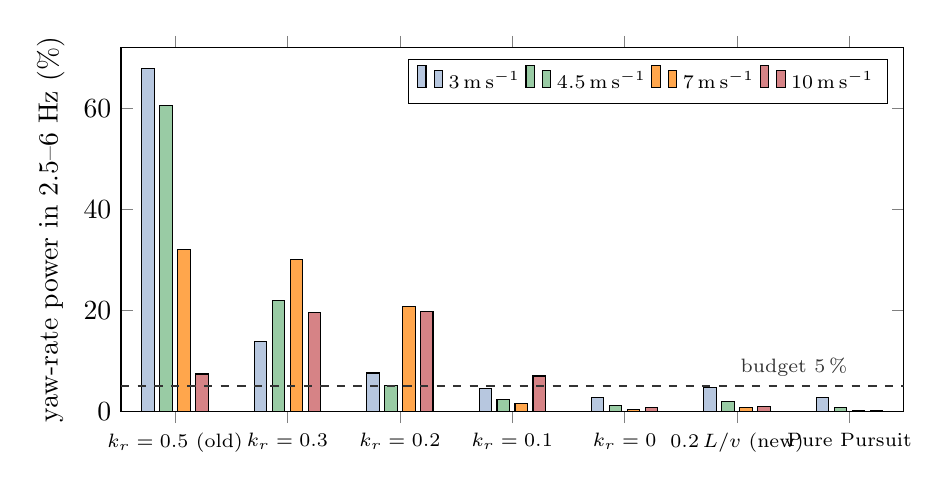
\begin{tikzpicture}
\begin{axis}[
  ybar, bar width=4.5pt, width=0.95\linewidth, height=6.2cm,
  ylabel={yaw-rate power in 2.5--6 Hz (\%)}, ymin=0, ymax=72,
  symbolic x coords={shipped,0.3,0.2,0.1,0,scaled,PP},
  xticklabels={{$k_r=0.5$ (old)},{$k_r=0.3$},{$k_r=0.2$},{$k_r=0.1$},{$k_r=0$},{$0.2\,L/v$ (new)},{Pure Pursuit}},
  xtick=data, x tick label style={font=\scriptsize, align=center},
  legend style={font=\scriptsize, at={(0.98,0.97)}, anchor=north east}, legend columns=4,
  enlarge x limits=0.08,
]
\addplot[fill=pp!40] coordinates {(shipped,67.9) (0.3,13.8) (0.2,7.6) (0.1,4.6) (0,2.7) (scaled,4.8) (PP,2.7)};
\addplot[fill=fix!60] coordinates {(shipped,60.6) (0.3,22.0) (0.2,5.1) (0.1,2.3) (0,1.2) (scaled,1.9) (PP,0.7)};
\addplot[fill=orange!70] coordinates {(shipped,32.1) (0.3,30.1) (0.2,20.8) (0.1,1.6) (0,0.4) (scaled,0.7) (PP,0.2)};
\addplot[fill=stan!70] coordinates {(shipped,7.4) (0.3,19.5) (0.2,19.7) (0.1,7.0) (0,0.7) (scaled,1.0) (PP,0.2)};
\legend{\SI{3}{\metre\per\second},\SI{4.5}{\metre\per\second},\SI{7}{\metre\per\second},\SI{10}{\metre\per\second}}
\draw[bud, dashed, thick] (rel axis cs:0,0.0694) -- node[pos=0.86, above, font=\scriptsize]{budget 5\,\%} (rel axis cs:1,0.0694);
\end{axis}
\end{tikzpicture}
\caption{Oscillation against the yaw-rate gain, closed-loop model with the HIL delays. At
\SI{10}{\metre\per\second} the old gain shows little band power only because the steering
sits on the rate limit 80\,\% of the time (\cref{tab:sweep}).}
\label{fig:sweep}
\end{figure}

\begin{table}[h]
\centering\small
\begin{tabular}{@{}lrrrrrr@{}}
\toprule
Lateral controller & \multicolumn{3}{c}{Ticks at the rate limit (\%)} & \multicolumn{3}{c}{Tracking error RMS (m)} \\
\cmidrule(lr){2-4}\cmidrule(l){5-7}
 & \SI{4.5}{\metre\per\second} & 7 & 10 & \SI{4.5}{\metre\per\second} & 7 & 10 \\
\midrule
Stanley, $k_r = 0.5$ (old) & 71.2 & 77.8 & 80.1 & 0.319 & 0.404 & 0.514 \\
Stanley, $k_r = 0.2$ & 0.4 & 37.5 & 71.8 & 0.272 & 0.316 & 0.299 \\
Stanley, $k_r = 0$ & 0.2 & 1.4 & 7.9 & 0.224 & 0.234 & 0.242 \\
\textbf{Stanley, $k_r = 0.2\,L/v$ (new)} & \textbf{0.2} & \textbf{1.5} & \textbf{7.2} & \textbf{0.240} & \textbf{0.249} & \textbf{0.242} \\
Pure Pursuit & 0.2 & 0.4 & 1.3 & 0.262 & 0.323 & 0.364 \\
\bottomrule
\end{tabular}
\caption{The same runs. $k_r=0$ is as good in this kinematic model, but a July note records
that the full sim, which has tyre dynamics, limit-cycled without yaw damping at a
higher cross-track gain. The scaled gain keeps the damping at a loop gain the delay
tolerates.}
\label{tab:sweep}
\end{table}

%=====================================================================
\section{Delay compensation: implemented, left off}\label{sec:delayresult}
%=====================================================================
With the corrected gain, the remaining question is whether steering for the predicted pose
(\cref{eq:predict}) helps. The model says it does not:
\begin{itemize}
\item Removing the actuation delay altogether does not reduce tracking error:
\begin{itemize}
\item new Stanley: \SI{0.240}{\metre} with the delay, \SI{0.248}{\metre} without, at
\SI{4.5}{\metre\per\second}; \SI{0.242}{} against \SI{0.276}{\metre} at
\SI{10}{\metre\per\second};
\item Pure Pursuit: \SI{0.262}{} against \SI{0.273}{\metre}, and \SI{0.364}{} against
\SI{0.423}{\metre}.
\end{itemize}
Both controllers already look ahead (look-ahead $L_d$, front axle at $L$) much further
than the car moves in \SI{45}{\milli\second} (\SI{0.2}{}--\SI{0.45}{\metre}).
\item Prediction adds more preview, so the car turns in earlier and cuts corners
(\cref{tab:delay}). It does lower the time at the rate limit at high speed.
\item A first version predicted with the measured yaw rate. It was worse, because that
yaw rate is itself \SI{55}{\milli\second} old.
\end{itemize}

\begin{table}[h]
\centering\small
\begin{tabular}{@{}lrrrrrrrr@{}}
\toprule
$\tau$ & \multicolumn{4}{c}{Stanley (new), error RMS (m)} & \multicolumn{4}{c}{Pure Pursuit, error RMS (m)} \\
\cmidrule(lr){2-5}\cmidrule(l){6-9}
(ms) & 4.5 & 7 & 10 & \SI{12}{\metre\per\second} & 4.5 & 7 & 10 & \SI{12}{\metre\per\second} \\
\midrule
0 & \textbf{0.240} & \textbf{0.249} & \textbf{0.242} & 0.276 & \textbf{0.262} & \textbf{0.323} & \textbf{0.364} & \textbf{0.354} \\
25 & 0.246 & 0.260 & 0.267 & \textbf{0.270} & 0.268 & 0.339 & 0.395 & 0.391 \\
50 & 0.253 & 0.274 & 0.294 & 0.301 & 0.275 & 0.357 & 0.431 & 0.433 \\
75 & 0.262 & 0.291 & 0.327 & 0.350 & 0.282 & 0.378 & 0.472 & 0.491 \\
\bottomrule
\end{tabular}
\caption{Command-history prediction (\cref{eq:predict}) in the closed-loop model.
Ticks at the rate limit, new Stanley at \SI{12}{\metre\per\second}: 12.2\,\% at
$\tau=0$, 5.8\,\% at \SI{50}{\milli\second}.}
\label{tab:delay}
\end{table}

The compensator stays in the code (C and Python, tested equal) behind
\texttt{latency\_comp\_s}. It becomes worth testing when the actuation delay grows (the
STM32 path will change it) or above \SI{10}{\metre\per\second}, where it reduces steering
saturation.

%=====================================================================
\section{Longitudinal control}
%=====================================================================

\subsection{Speed setpoint}
Regen is the only service brake and it is power limited: with $P = \SI{11}{\kilo\watt}$
(the pack's charge limit), $m = \SI{275}{\kilo\gram}$ and $a_d = \SI{4}{\metre\per\second\squared}$,
\begin{equation}
a(v) = \min\!\left(a_d,\ \frac{P}{m v}\right), \qquad v^* = \frac{P}{m a_d} = \SI{10}{\metre\per\second}.
\end{equation}
The fastest speed now from which the car can still be at $v_e$ after $s$ metres of
braking comes from integrating $v\,\mathrm{d}v = -a(v)\,\mathrm{d}s$. Below $v^*$ the
deceleration is constant; above it $m v^2\,\mathrm{d}v = -P\,\mathrm{d}s$:
\begin{equation}
v_b(v_e, s) =
\begin{cases}
\sqrt{v_e^2 + 2 a_d s} & v_e < v^*,\ s \le s_c, \\[2pt]
\left(v^{*3} + \frac{3P}{m}(s - s_c)\right)^{1/3} & v_e < v^*,\ s > s_c, \\[2pt]
\left(v_e^3 + \frac{3P}{m}s\right)^{1/3} & v_e \ge v^*,
\end{cases}
\qquad s_c = \frac{v^{*2} - v_e^2}{2 a_d}.
\label{eq:vb}
\end{equation}
The regen ramp-up and the PI lag cost distance before braking bites:
$\ell = \max(0, v_x)\,t_\ell$ with $t_\ell = \SI{0.3}{\second}$. Every path point $i$ ahead
of the car is a corner with grip-limited speed $\sqrt{a_{\text{lat}}/|\kappa_i|}$
($a_{\text{lat}} = \SI{3}{\metre\per\second\squared}$). The end of the visible path counts as an
unseen hairpin of radius $R_u = \SI{4.5}{\metre}$ (off in acceleration). The stop target
counts as a corner of speed zero. Then
\begin{equation}
v_{\text{set}} = \max\!\Big(0,\ \min\Big\{ v_{\max},\
  \min_{i} v_b\!\big(\sqrt{a_{\text{lat}}/|\kappa_i|},\ s_i - s_0 - \ell\big),\
  v_b\!\big(\sqrt{a_{\text{lat}} R_u},\ s_{N-1} - s_0 - \ell\big),\
  v_b(0,\ d_{\text{stop}} - \ell) \Big\}\Big).
\end{equation}

\subsection{Speed tracking}
The measured speed is conditioned before the PI. A plausibility clamp limits each step to
$a_{\max} T_s$ (with $a_{\max} = \SI{20}{\metre\per\second\squared}$), against the
previous clamped sample. An exponential filter
$\hat v \leftarrow \hat v + \alpha (v - \hat v)$, with
$\alpha = T_s / (\tau_v + T_s) = 0.143$ ($\tau_v = \SI{0.15}{\second}$), smooths it. The
tracked speed is $\max(\hat v, v_{\text{clamped}})$, which removes the filter lag while
accelerating. Then
\begin{equation}
e = v_{\text{set}} - v_{\text{tr}}, \quad
u = \sat_{[-1,1]}\!\left(k_p e + k_i \textstyle\int e\right), \quad
k_p = 0.5,\ k_i = \SI{0.05}{\per\second},
\end{equation}
with conditional integration (the integral holds while $u$ saturates). The output splits
with a deadband $d = 0.05$: throttle $= \min(u, u_{\max})$ if $u \ge d$, regen $= -u$ if
$u \le -d$, coast otherwise.

\subsection{Finish stop}
The stop latches on the first array of at least two big-orange cones that satisfies all
of these:
\begin{itemize}
\item the car has travelled at least \SI{30}{\metre};
\item SLAM says this is the closing lap;
\item the car has travelled at least \SI{30}{\metre} since the closing lap began.
\end{itemize}
The cones' centroid, moved into the map frame with the current SLAM pose, is the anchor.
The target is \SI{8}{\metre} past it along the approach direction $\hat u$. The distance
left is $d_{\text{stop}} = (p_t - p)\cdot\hat u$, which becomes negative past the target;
in skidpad it is the straight-line distance to the anchor.

%=====================================================================
\section{Output stage}
%=====================================================================
\begin{itemize}
\item \textbf{Sign.} The published steering is $-u$: positive to the right, the vehicle
interface's convention.
\item \textbf{Start-up cap.} Over the first metre travelled, $|u|$ is capped at
$0.3 + 0.7\,s_{\text{trav}}$. The first paths are often off-axis.
\item \textbf{Slew limits} (per second, applied per tick):
\begin{itemize}
\item throttle up 2.0, down 8.0;
\item regen 3.33;
\item steering 5.0, that is \num{0.125} per tick, or full lock from centre in
\SI{0.2}{\second}.
\end{itemize}
These rates set the phase lag that brought the limit cycle of \cref{sec:stability} down
from \SI{4.5}{} to \SI{4}{\hertz}.
\end{itemize}

%=====================================================================
\section{Measured performance (HIL v10, before the fixes)}
%=====================================================================
Ground truth from the sim, recorded on the HIL computer. ``Offset'' is half the
difference between the distances to the blue and yellow boundaries. ``Clearance'' is the
distance from the car's reference point to the nearest cone centre; the car's half-width
is \SI{0.7}{\metre}.

\begin{table}[h]
\centering\small
\resizebox{\linewidth}{!}{\begin{tabular}{@{}llrrrrrr@{}}
\toprule
Mission & Lateral & Cones hit & $\bar v$ (m/s) & $|a_y|_{p95}$ (m/s$^2$) & Offset RMS (m) & Clearance min (m) & Reversals /\SI{100}{\metre} \\
\midrule
Acceleration & PP & 0 & 10.40 & 2.82 & 0.10 & 1.35 & 2.6 \\
Skidpad & Stanley & 4 & 4.24 & 4.64 & -- & 0.63 & 26.6 \\
Autocross A & Stanley & 6 & 4.56 & 2.35 & 0.33 & 0.54 & 146.9 \\
Autocross B & Stanley & 4 & 4.64 & 2.19 & 0.33 & 0.62 & 137.9 \\
Autocross C & Stanley & 7 & 4.56 & 2.15 & 0.34 & 0.53 & 125.8 \\
Autocross D & Stanley & 3 & 4.39 & 2.12 & 0.36 & 0.52 & 130.2 \\
Trackdrive A & PP & 0 & 4.84 & 2.87 & 0.12 & 0.97 & 7.7 \\
Trackdrive B & PP & 0 & 4.88 & 2.64 & 0.12 & 1.04 & 7.7 \\
Trackdrive C & PP & 0 & 4.85 & 2.49 & 0.12 & 0.94 & 7.9 \\
Trackdrive D & PP & 0 & 4.80 & 2.55 & 0.14 & 0.93 & 10.1 \\
\bottomrule
\end{tabular}}
\caption{Control baseline, HIL v10 (pipeline c488839). Trackdrive covers 10 laps,
3.5--\SI{5.4}{\kilo\metre} per track.}
\label{tab:baseline}
\end{table}

\begin{figure}[h]
\centering
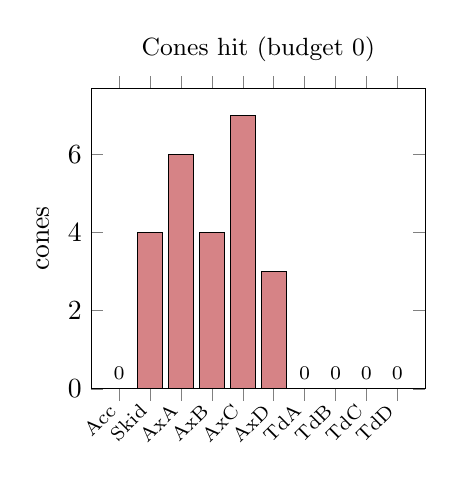
\begin{tikzpicture}
\begin{axis}[
  ybar, bar width=9pt, width=0.48\linewidth, height=5.4cm, ymin=0,
  title={\small Cones hit (budget 0)}, ylabel={cones},
  symbolic x coords={Acc,Skid,AxA,AxB,AxC,AxD,TdA,TdB,TdC,TdD}, xtick={Acc,Skid,AxA,AxB,AxC,AxD,TdA,TdB,TdC,TdD},
  x tick label style={font=\scriptsize, rotate=45, anchor=east}, bar shift=0pt,
]
\addplot[fill=stan!70] coordinates {(Skid,4) (AxA,6) (AxB,4) (AxC,7) (AxD,3)};
\addplot[fill=pp!60, nodes near coords, nodes near coords style={font=\scriptsize}] coordinates {(Acc,0) (TdA,0) (TdB,0) (TdC,0) (TdD,0)};
\end{axis}
\end{tikzpicture}\hfill
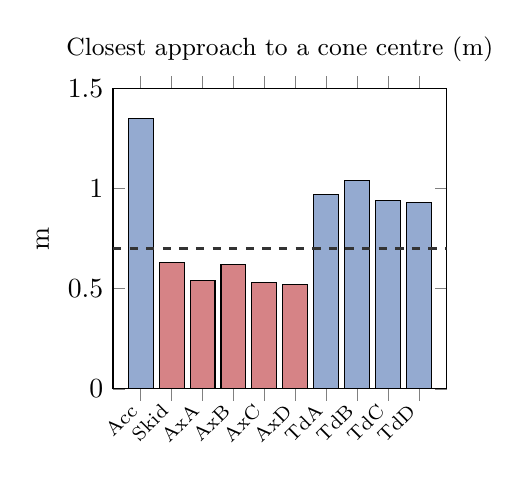
\begin{tikzpicture}
\begin{axis}[
  ybar, bar width=9pt, width=0.48\linewidth, height=5.4cm, ymin=0, ymax=1.5,
  title={\small Closest approach to a cone centre (m)}, ylabel={m},
  symbolic x coords={Acc,Skid,AxA,AxB,AxC,AxD,TdA,TdB,TdC,TdD}, xtick={Acc,Skid,AxA,AxB,AxC,AxD,TdA,TdB,TdC,TdD},
  x tick label style={font=\scriptsize, rotate=45, anchor=east}, bar shift=0pt,
]
\addplot[fill=stan!70] coordinates {(Skid,0.63) (AxA,0.54) (AxB,0.62) (AxC,0.53) (AxD,0.52)};
\addplot[fill=pp!60] coordinates {(Acc,1.35) (TdA,0.97) (TdB,1.04) (TdC,0.94) (TdD,0.93)};
\draw[bud, dashed, thick] (rel axis cs:0,0.467) -- (rel axis cs:1,0.467);
\end{axis}
\end{tikzpicture}
\caption{Red: Stanley missions. Blue: Pure Pursuit missions. Same tracks for autocross and
trackdrive. Dashed: the car's half-width, \SI{0.7}{\metre}; below it a cone touches the body.}
\label{fig:baseline}
\end{figure}

\paragraph{What else the baseline shows.}
\begin{itemize}
\item Trackdrive averages \SI{4.84}{\metre\per\second} against $v_{\max} = 5$, so the
speed cap sets lap time, not grip. The 95th percentile of lateral acceleration is
\SIrange{2.5}{2.9}{\metre\per\second\squared}, against the \SI{3}{} the setpoint allows.
\item Skidpad reached \SI{6.9}{\metre\per\second} against $v_{\max} = 5$. This is still
open.
\end{itemize}

%=====================================================================
\section{Measured performance after the fixes (HIL v12)}\label{sec:v12}
%=====================================================================
The same 10 missions on pipeline \texttt{b1a2bf9} (14 November 2026): control in C, the
speed-scaled Stanley gain (\cref{eq:kr}), the \texttt{final\_lap} race fix (SLAM recreates
its latched writers every mission) and centreline smoothing 0.05. All 10 missions finished
(v11, C control with the old gain, failed acceleration and trackdrive D).

\begin{table}[h]
\centering\small
\resizebox{\linewidth}{!}{%
\begin{tabular}{@{}llrrrrrr@{}}
\toprule
Mission & Lateral & Cones hit & Reversals /\SI{100}{\metre} & At rate limit (\%) & Clearance min (m) & Offset RMS (m) & $\bar v$ (m/s) \\
\midrule
Acceleration & PP & 0 \,(0) & 5.8 \,(2.6) & 0.0 \,(0.0) & 1.42 \,(1.35) & 0.04 \,(0.10) & 10.31 \\
Skidpad & Stanley & 1 \,(4) & 6.0 \,(26.6) & 0.1 \,(11.3) & 0.73 \,(0.63) & -- & 4.41 \\
Autocross A & Stanley & 1 \,(6) & 25.7 \,(146.9) & 0.5 \,(16.2) & 0.73 \,(0.54) & 0.23 \,(0.33) & 4.58 \\
Autocross B & Stanley & 0 \,(4) & 21.9 \,(137.9) & 0.7 \,(12.8) & 0.89 \,(0.62) & 0.19 \,(0.33) & 4.72 \\
Autocross C & Stanley & 1 \,(7) & 23.3 \,(125.8) & 0.8 \,(11.0) & 0.76 \,(0.53) & 0.22 \,(0.34) & 4.64 \\
Autocross D & Stanley & 0 \,(3) & 27.8 \,(130.2) & 0.7 \,(10.6) & 0.79 \,(0.52) & 0.23 \,(0.36) & 4.44 \\
Trackdrive A & PP & 0 \,(0) & 11.1 \,(7.7) & 0.7 \,(0.2) & 1.04 \,(0.97) & 0.12 \,(0.12) & 4.75 \\
Trackdrive B & PP & 0 \,(0) & 7.9 \,(7.7) & 0.3 \,(0.3) & 1.06 \,(1.04) & 0.10 \,(0.12) & 4.85 \\
Trackdrive C & PP & 0 \,(0) & 13.2 \,(7.9) & 1.5 \,(0.6) & 1.03 \,(0.94) & 0.12 \,(0.12) & 4.78 \\
Trackdrive D & PP & 0 \,(0) & 13.9 \,(10.1) & 1.5 \,(0.9) & 1.06 \,(0.93) & 0.12 \,(0.14) & 4.72 \\
\bottomrule
\end{tabular}}
\caption{HIL v12, with v10 in brackets. Per-mission windows for v12 come from the mission
start messages in the bag; v10 used manual windows.}
\label{tab:v12}
\end{table}

\begin{figure}[!htbp]
\centering
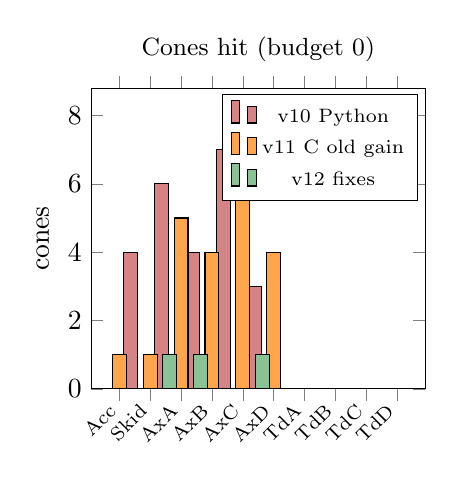
\begin{tikzpicture}
\begin{axis}[
  ybar, bar width=5pt, width=0.48\linewidth, height=5.4cm, ymin=0,
  title={\small Cones hit (budget 0)}, ylabel={cones},
  symbolic x coords={Acc,Skid,AxA,AxB,AxC,AxD,TdA,TdB,TdC,TdD},
  xtick={Acc,Skid,AxA,AxB,AxC,AxD,TdA,TdB,TdC,TdD},
  x tick label style={font=\scriptsize, rotate=45, anchor=east},
  legend style={font=\scriptsize}, legend columns=1,
]
\addplot[fill=stan!70] coordinates {(Acc,0) (Skid,4) (AxA,6) (AxB,4) (AxC,7) (AxD,3) (TdA,0) (TdB,0) (TdC,0) (TdD,0)};
\addplot[fill=orange!70] coordinates {(Acc,1) (Skid,1) (AxA,5) (AxB,4) (AxC,8) (AxD,4) (TdA,0) (TdB,0) (TdC,0) (TdD,0)};
\addplot[fill=fix!70] coordinates {(Acc,0) (Skid,1) (AxA,1) (AxB,0) (AxC,1) (AxD,0) (TdA,0) (TdB,0) (TdC,0) (TdD,0)};
\legend{v10 Python, v11 C old gain, v12 fixes}
\end{axis}
\end{tikzpicture}\hfill
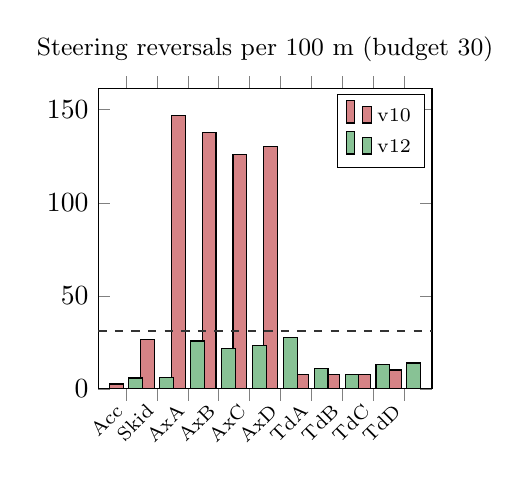
\begin{tikzpicture}
\begin{axis}[
  ybar, bar width=5pt, width=0.48\linewidth, height=5.4cm, ymin=0,
  title={\small Steering reversals per 100 m (budget 30)},
  symbolic x coords={Acc,Skid,AxA,AxB,AxC,AxD,TdA,TdB,TdC,TdD},
  xtick={Acc,Skid,AxA,AxB,AxC,AxD,TdA,TdB,TdC,TdD},
  x tick label style={font=\scriptsize, rotate=45, anchor=east},
  legend style={font=\scriptsize},
]
\addplot[fill=stan!70] coordinates {(Acc,2.6) (Skid,26.6) (AxA,146.9) (AxB,137.9) (AxC,125.8) (AxD,130.2) (TdA,7.7) (TdB,7.7) (TdC,7.9) (TdD,10.1)};
\addplot[fill=fix!70] coordinates {(Acc,5.8) (Skid,6.0) (AxA,25.7) (AxB,21.9) (AxC,23.3) (AxD,27.8) (TdA,11.1) (TdB,7.9) (TdC,13.2) (TdD,13.9)};
\legend{v10, v12}
\draw[bud, dashed, thick] (rel axis cs:0,0.193) -- (rel axis cs:1,0.193);
\end{axis}
\end{tikzpicture}
\caption{HIL v10 against v12, per mission. Dashed: the budget, 30 reversals per 100 m.}
\label{fig:v12}
\end{figure}

\paragraph{What changed.}
\begin{itemize}
\item \textbf{Stanley:} the \SI{4}{\hertz} weave is gone. Autocross steering reversals fell
about five times, time at the rate limit from 11--16\,\% to under 1\,\%, and the closest
approach to a cone rose from 0.52--0.62 to 0.73--0.89\,m, all above the car's half-width.
Cones hit fell from 24 to 3.
\item \textbf{Trackdrive (Pure Pursuit):} slightly busier steering (reversals 8--14 per
\SI{100}{\metre}, was 8--10; full lock about 2\,\% of the time on tracks A and C), most likely
because the less-smoothed path follows the cones more closely. Path error fell from 0.19 to
0.13\,m RMS and clearance rose. Mean speed fell slightly, 4.72--4.85 against
4.80--4.88\,m/s.
\item \textbf{Core 7:} mean 45.7\,\%, p95 51.9\,\% (v10: 94.3\,\% and 100\,\%).
\item \textbf{Skidpad} peaked at \SI{5.02}{\metre\per\second} (v10: 6.9 against a cap of 5);
not investigated.
\end{itemize}
Trackdrive D ran at 0.94 of real time because a CI job shared the HIL computer; its
throttle/regen switching (330, v10: 180) may partly come from that.

%=====================================================================
\section{Going past \SI{10}{\metre\per\second}}
%=====================================================================
Three limits come before the control law. They follow from \cref{eq:vb}.

\paragraph{Sight distance.} The car must reach $\sqrt{a_{\text{lat}} R_u} =
\SI{3.67}{\metre\per\second}$ by the end of the visible path, with the latency loss
$\ell = 0.3\,v$. Solving $v = v_b(3.67,\ s_{\text{path}} - 0.3 v)$ by fixed point:

\begin{center}\small
\begin{tabular}{@{}lrrrrrr@{}}
\toprule
Visible path (m) & 11.6 (today) & 15 & 20 & 30 & 40 & 60 \\
Speed cap (m/s) & 9.2 & 10.4 & 11.9 & 14.1 & 15.8 & 18.4 \\
\bottomrule
\end{tabular}
\end{center}

On mapped laps, planning from the SLAM map lifts this cap: the horizon becomes the whole
lap.

\paragraph{Grip setting.} Corner speed is $\sqrt{a_{\text{lat}} R}$. At \SI{3}{\metre\per\second\squared}
that is \SI{5.2}{\metre\per\second} for $R = \SI{9}{\metre}$; at 10--\SI{14}{\metre\per\second\squared},
typical of FS cars, it is 9.5--\SI{11.2}{\metre\per\second}. The value should be measured,
not assumed.

\paragraph{Regen braking.} $a(v)$ falls to \SI{2.67}{\metre\per\second\squared} at
\SI{15}{\metre\per\second} and \SI{2.0}{} at \SI{20}{}. Braking from 15 to
\SI{5}{\metre\per\second} takes \SI{29.2}{\metre} (plus \SI{4.5}{\metre} of latency); from
20, \SI{67.7}{\metre}.

\paragraph{Lateral.} With the scaled gain, the closed-loop model stays stable to
\SI{12}{\metre\per\second} (\cref{tab:sweep,tab:delay}). Above about
\SI{10}{\metre\per\second} in tight corners the kinematic model stops being valid (tyre
slip). The next step there is a dynamic bicycle model with speed-scheduled LQR gains,
which fits the STM32H7.

%=====================================================================
\section{Implementation}
%=====================================================================
\begin{table}[h]
\centering\small
\resizebox{\linewidth}{!}{\begin{tabular}{@{}lll@{}}
\toprule
Part & File & Notes \\
\midrule
Controller & \texttt{control\_cpp/src/control\_core.c} & C99, \texttt{<math.h>}; 66~KB state (17~KB with smaller buffers) \\
ROS 2 node & \texttt{control\_cpp/src/control\_node.cpp} & same topics, QoS and parameters as Python \\
Reference & \texttt{control/control/*.py} & \texttt{DV\_CONTROL=python} to run it \\
Equivalence tests & \texttt{control/test/test\_control\_core\_c.py} & each piece, plus closed-loop node runs \\
Parameters & \texttt{bringup/config/params.yaml} & \texttt{stanley\_yaw\_rate\_loop\_gain}, \texttt{latency\_comp\_s} \\
\bottomrule
\end{tabular}}
\end{table}

\begin{figure}[!htbp]
\centering
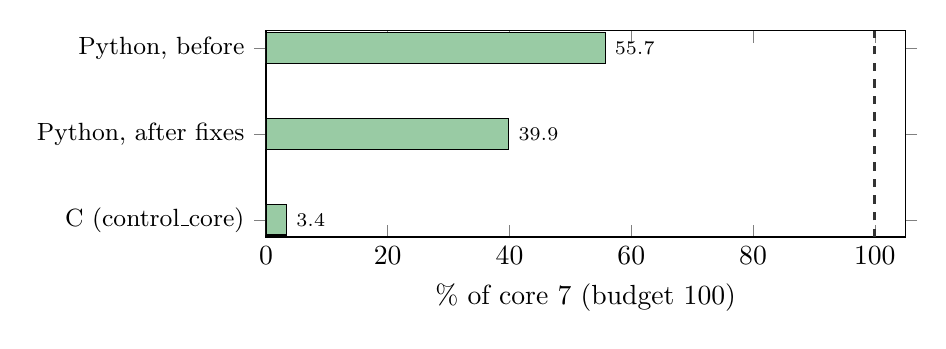
\begin{tikzpicture}
\begin{axis}[
  xbar, bar width=11pt, width=0.8\linewidth, height=4.2cm, xmin=0, xmax=105,
  xlabel={\% of core 7 (budget 100)},
  symbolic y coords={C,Pyfix,Py}, ytick=data,
  yticklabels={C (control\_core),{Python, after fixes},{Python, before}},
  y tick label style={font=\small}, nodes near coords, nodes near coords style={font=\scriptsize},
]
\addplot[fill=fix!60] coordinates {(3.4,C) (39.9,Pyfix) (55.7,Py)};
\draw[bud, dashed, thick] (rel axis cs:0.952,0) -- (rel axis cs:0.952,1);
\end{axis}
\end{tikzpicture}
\caption{Control alone on core 7, bag replay. ``Before'' is after 10 missions; the others
use a fresh node.}
\end{figure}

\paragraph{Core 7 in HIL.} The same 10 missions with the C node (HIL \texttt{hil\_v11\_cctrl},
14 November 2026, pipeline \texttt{ee729f0}, before the Stanley fix), against the Python
node (v10). Core 7 runs control, the odometry filter and the network interrupts.

\begin{figure}[!htbp]
\centering
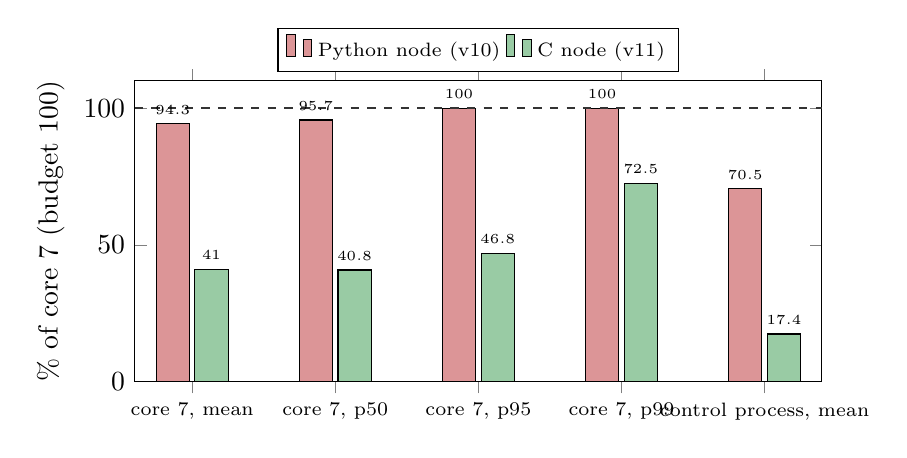
\begin{tikzpicture}
\begin{axis}[
  ybar, bar width=12pt, width=0.85\linewidth, height=5.4cm, ymin=0, ymax=110,
  ylabel={\% of core 7 (budget 100)}, symbolic x coords={mean,p50,p95,p99,ctl}, xtick=data,
  xticklabels={{core 7, mean},{core 7, p50},{core 7, p95},{core 7, p99},{control process, mean}},
  x tick label style={font=\scriptsize}, nodes near coords, nodes near coords style={font=\tiny},
  legend style={font=\scriptsize, at={(0.5,1.03)}, anchor=south}, legend columns=2,
]
\addplot[fill=stan!60] coordinates {(mean,94.3) (p50,95.7) (p95,100) (p99,100) (ctl,70.5)};
\addplot[fill=fix!60] coordinates {(mean,41.0) (p50,40.8) (p95,46.8) (p99,72.5) (ctl,17.4)};
\legend{Python node (v10), C node (v11)}
\draw[bud, dashed, thick] (rel axis cs:0,0.909) -- (rel axis cs:1,0.909);
\end{axis}
\end{tikzpicture}
\caption{Core 7 load over the whole HIL session, 1~Hz samples (8194 and 9064). The C
node in the full loop costs more than in the bag replay (17\,\% against 3.4\,\%): there it
also carries the rclcpp executor, the message conversions and the logging.}
\end{figure}

Cones hit were unchanged (Stanley missions 21 against 24, Pure Pursuit trackdrive 0), as
expected without the gain fix. Two runs failed for reasons outside the control law:
\begin{itemize}
\item \textbf{Acceleration} hit a cone at \SI{12.5}{\second} (\SI{6.9}{\metre\per\second}), left
the track and timed out. This matches the open acceleration regression of the
perception changes on this branch; it needs a rerun before it is pinned on control.
\item \textbf{Trackdrive D} stopped after lap 1. Between missions, control got this
mission's \texttt{/slam/final\_lap = False} and then, \SI{75}{\milli\second} later, the previous
trackdrive's latched \texttt{True}, because SLAM's latched writer outlived the mission.
Fixed on both sides: SLAM recreates its latched writers on every activation, and control
ignores a rise of \texttt{final\_lap} before \texttt{stop\_latch\_min\_travel} (\SI{30}{\metre}).
\end{itemize}

\paragraph{Porting to the uDV.} The firmware compiles \texttt{control\_core.c} as is. It
feeds \texttt{ctrl\_node\_on\_odom} from its own odometry, and the path, pose and cones
from the Pi. It calls \texttt{ctrl\_node\_tick} at \SI{40}{\hertz}. The Cortex-M7 has a
double-precision FPU. Moving control there removes the relay and the network hop from the
command path and the \SI{55}{\milli\second} odometry filter from the yaw-rate path. That
raises $f_{180}$ in \cref{eq:loop} and widens the margin of every loop above.

\end{document}
